\label{sect:nucleus}


\begin{figure}
\centering
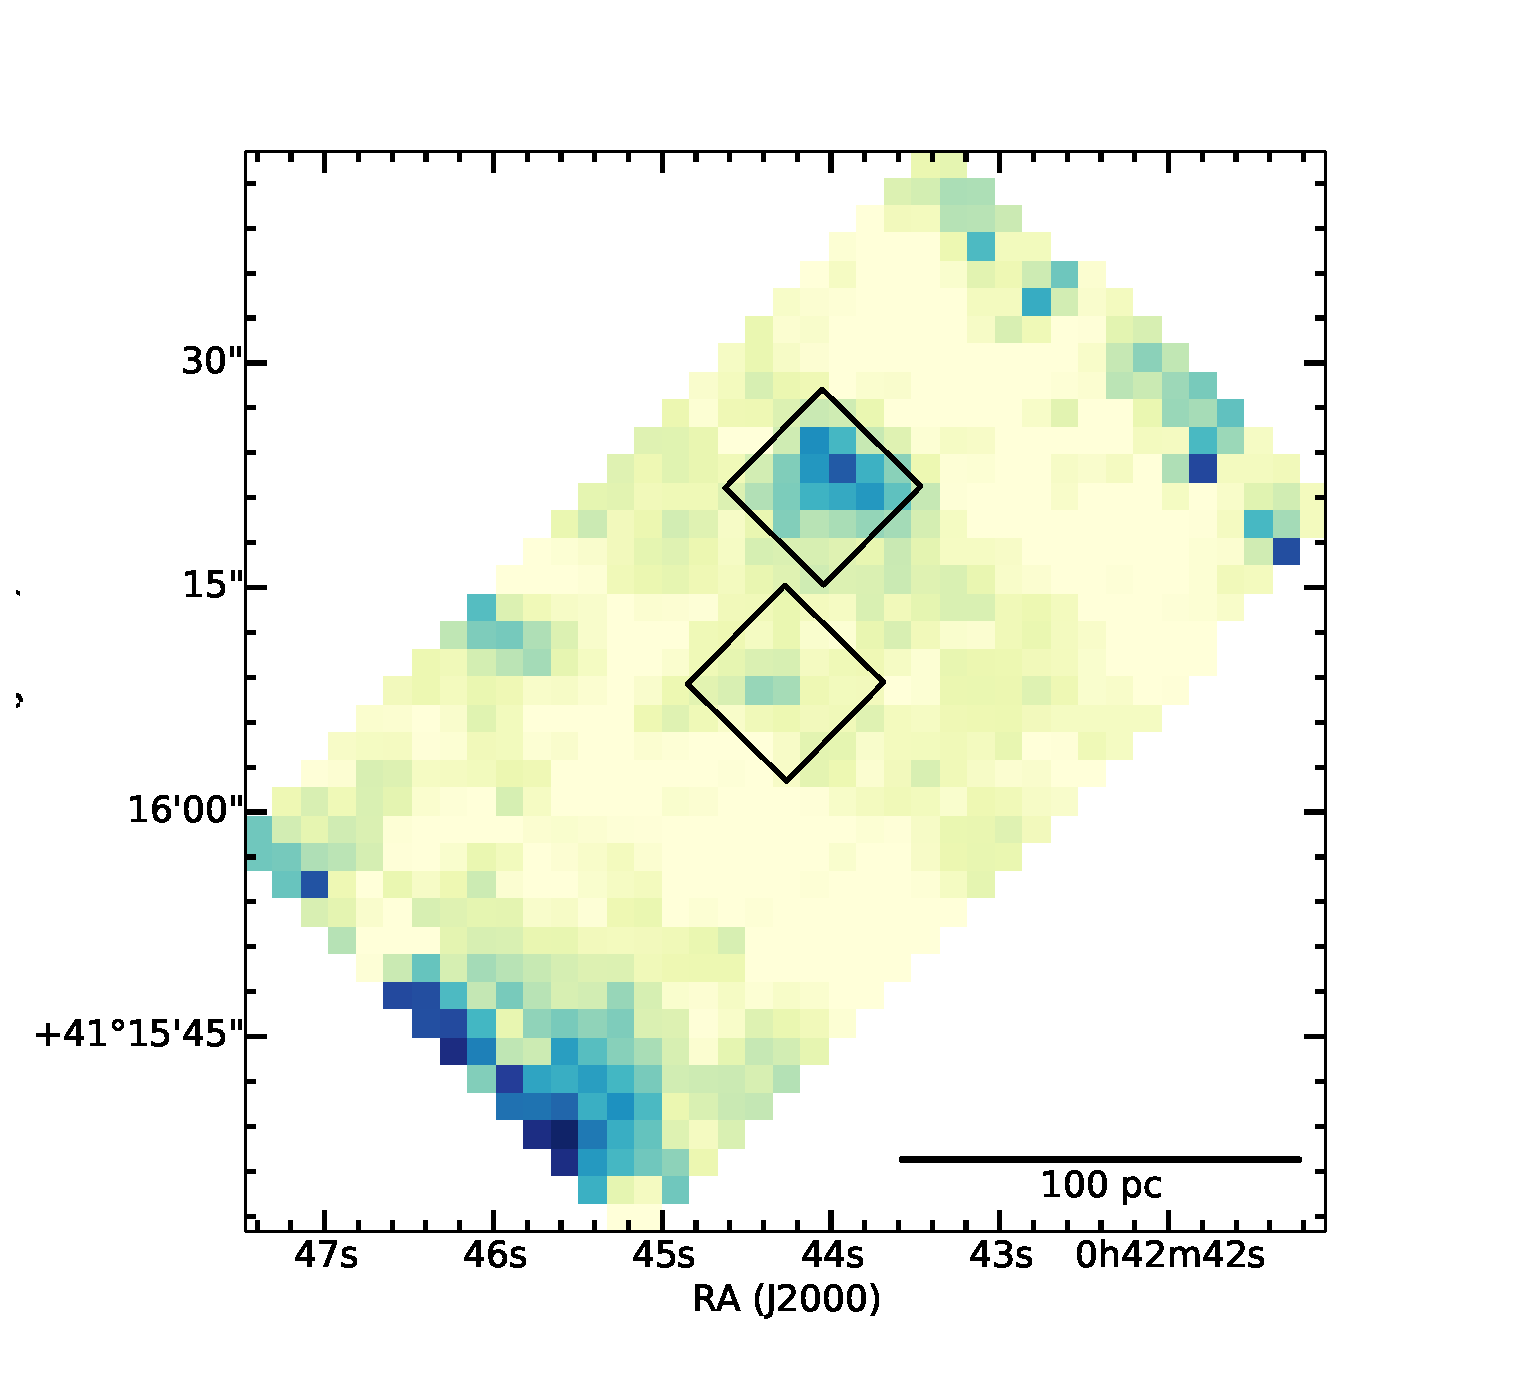
\includegraphics[scale = 0.25]{./fig10a.eps}
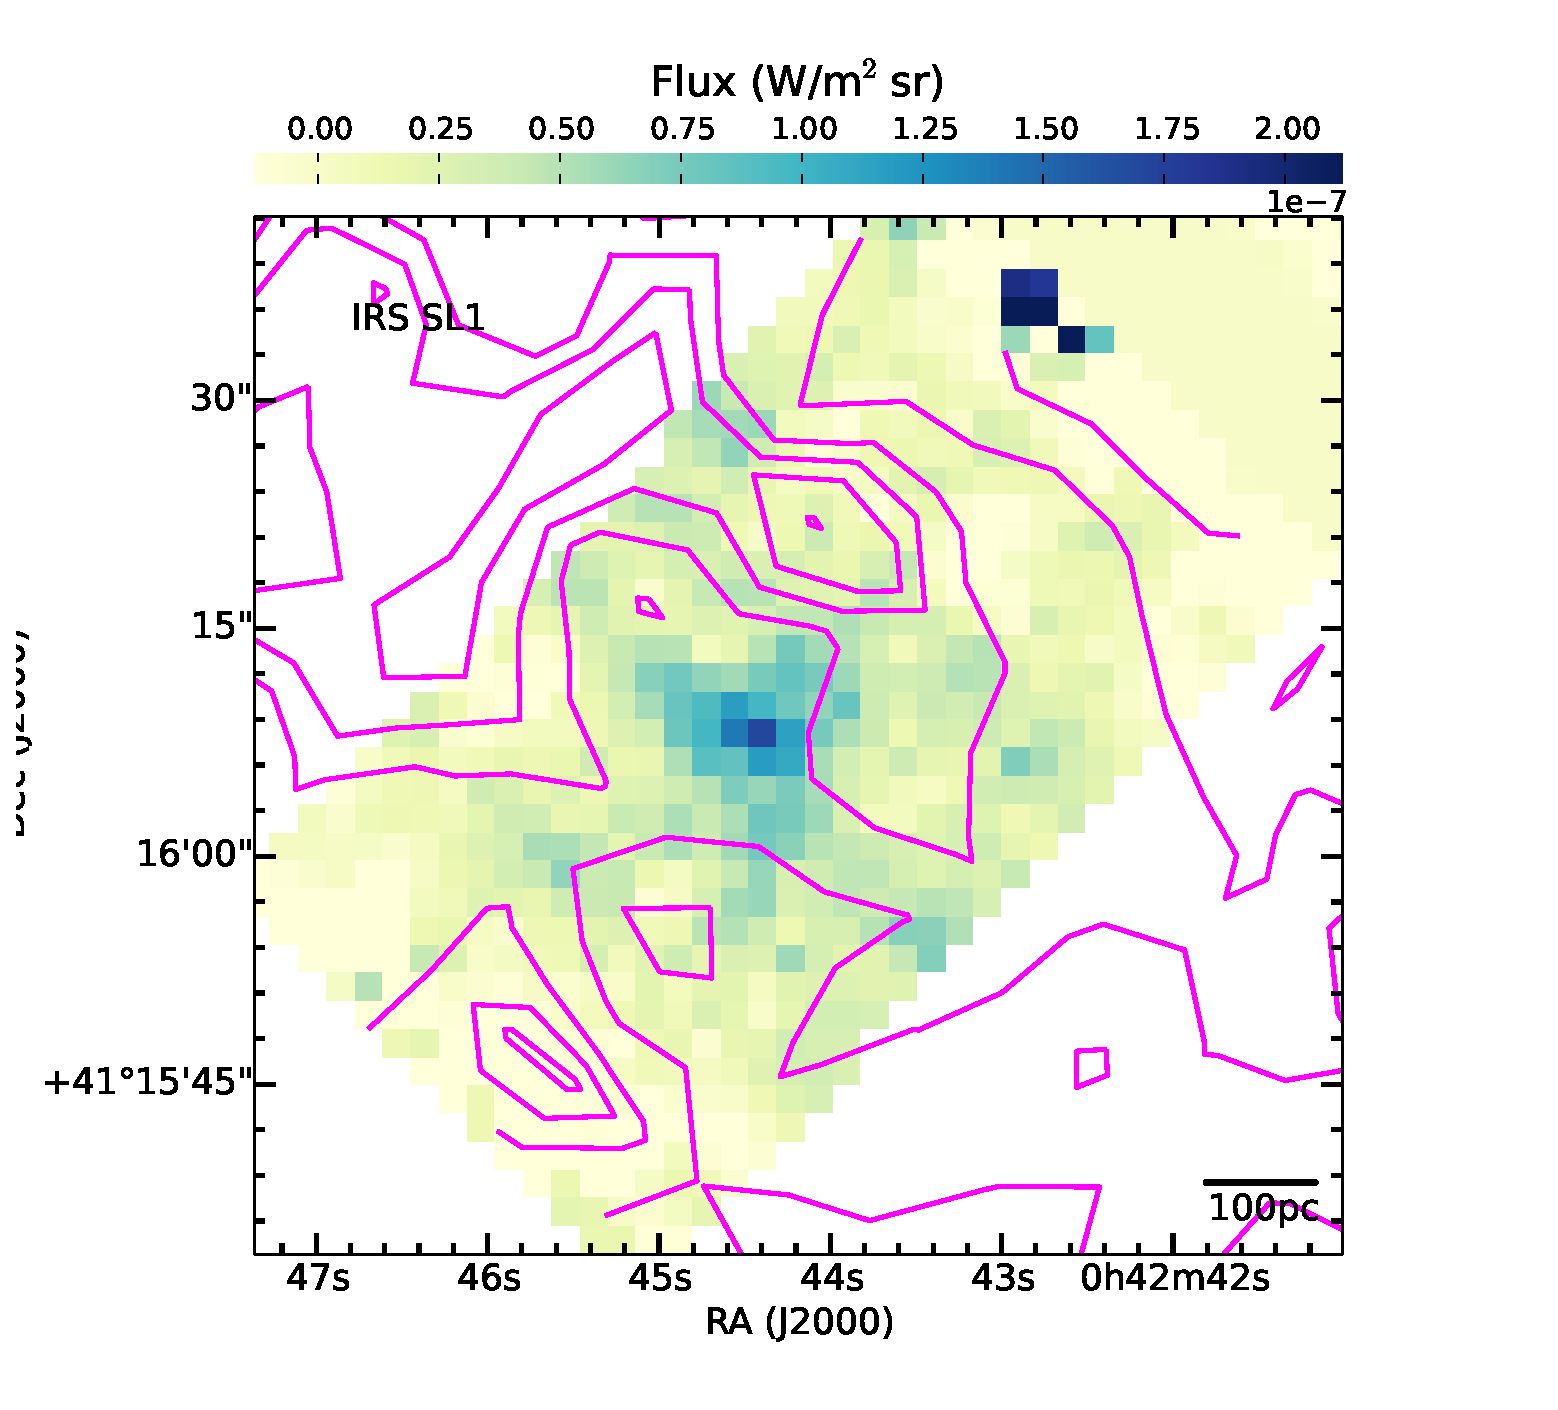
\includegraphics[scale = 0.25]{./fig10b.eps}
\caption{
Integrated strength of the 11.2~$\mu$m PAH emission (top) and the silicate emission (from 9 to 11~$\mu$m, continuum subtracted; bottom) 
around the nucleus of M31. 
The  two black boxes in the top panel are the 15\arcsec\ $\times$ 15\arcsec\ sub-apertures (centre and north region) used to extract spectra.  
The small white circle in the bottom panel shows a position halfway between the two components of the nucleus; these
components are separated by 0\farcs5, which is well below the IRS spatial resolution. The contours in the bottom panel indicate
the distribution of 3.6~$\mu$m luminosity, indicating the orientation of the M31 bulge.
}
\label{nuc11}
\end{figure}

Examining the {\em Spitzer}-IRS spectral data cube for the nuclear region, we noticed that different spectral features vary spatially within this region.
The 11.2~$\mu$m PAH emission is discrete and patchy (Figure \ref{nuc11}, top).  
Indeed, the majority of the 11.2~$\mu$m  PAH emission is from a region 15\arcsec\ north of the nucleus (00:42:43.947, +41:16:22.92) and not from 
the nucleus itself. Weaker 11.2~$\mu$m PAH emission is also found near the edge of the map peaking at 00:42:45.497, +41:15:43.97 and near 00:42:45.869; +41:16:11.38.
The locations of the two weaker 11.2~$\mu$m PAH emission peaks are also near positions exhibiting CO(2-1) line emission \citep[\#36 and 28 of][the strongest 11.2~$\mu$m PAH emission peak is outside the CO FOV]{Melchior2013}. 
On the other hand, the centre shows no PAH emission, but it does have clear silicate emission around 9.7~$\mu$m (Figure \ref{nuc11}, bottom).%
\footnote{The spatial resolution and pixel scale of the ISOCAM data are not sufficient to resolve the centre  and north regions.}
Although [NeIII] 15.5~$\mu$m line emission is strong at the three locations with 11.2~$\mu$m PAH emission and weak(er) at the nucleus, 
it is also present across the nuclear region and thus distinct from that of the silicate and PAH emission. 

Some structures seen in the optical near the M31 nucleus, such as the double nucleus and cluster of young stars, cannot be resolved with the data discussed here. The IRS spectral cubes have pixel sizes of 1\farcs8, and the SL PSF FWHM is 2.5--3\arcsec depending on the wavelength, while the two components of the nucleus are separated by only 0\farcs5 \citep{Bender2005}. However, the north 11.2~$\mu$m  PAH emission appear to be marginally spatially resolved: its radial profile has a full width at half maximum (FWHM) of 5--7\arcsec\ (corresponding to 19--27~pc).

% different spectra in nuclear area
To examine this spatial variation towards the nucleus in more detail, we extracted spectra from the centre and the North regions using  $9\arcsec \times 9\arcsec$ square apertures in addition to the full 30\arcsec $\times$ 50\arcsec\ M31 nuclear spectrum (further referred to as nuclear spectrum, north spectrum and full spectrum respectively), as shown in Figures~\ref{smithspec} and~\ref{fig:nuc_stellar}. Both spectra show a blue continuum and atomic fine-structure lines of Ne and S but they exhibit distinct dust emission consistent with the spatial maps: PAH emission is detected in the north spectrum while silicate emission is dominating in the nuclear spectrum.  In addition, weak H$_2$ emission is present at 17~$\mu$m in {\bf Els: in which spectra?}.

\begin{figure*}
\centering
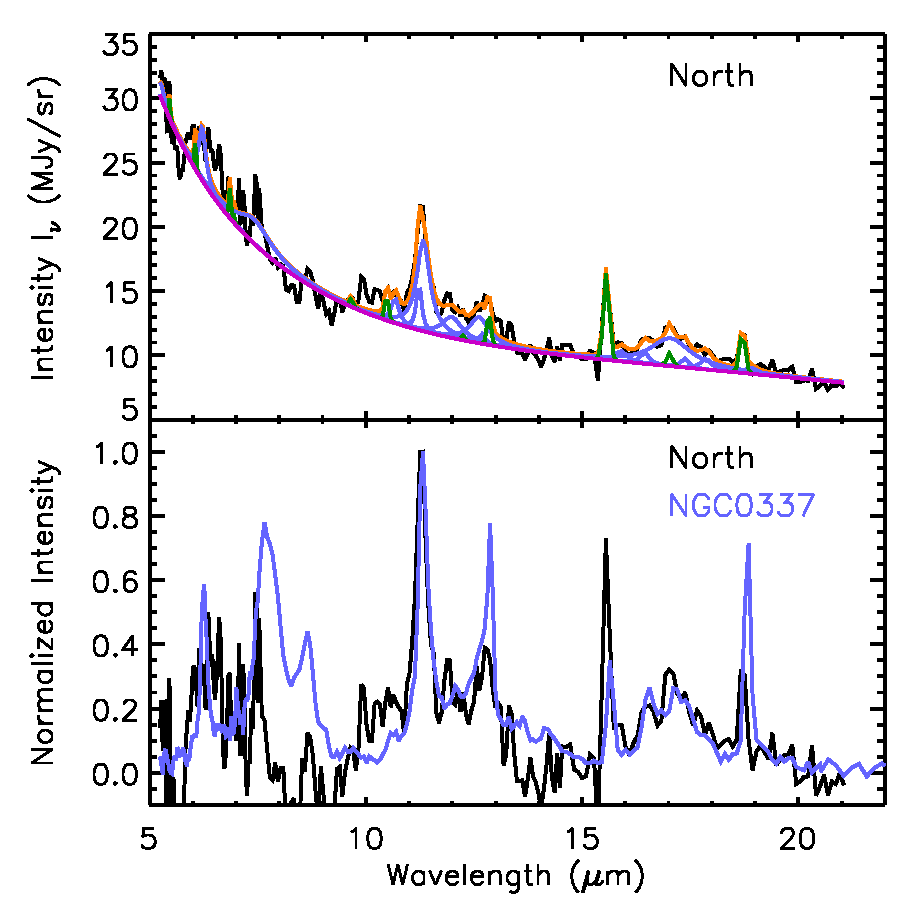
\includegraphics[height = 8 cm]{./fig11.eps}
\caption{Mid-infrared spectrum of the nucleus of M31 (blue; full spectrum) over-plotted with spectra extracted close to the nuclei of 6 nearby galaxies 
%which have AGN activity 
which have similar spectral shapes \citep{Smith:2007lr}. NGC 4552, NGC 1404 and NGC 4125 are elliptical galaxies and NGC 4594 and NGC 2841 are spiral galaxies. 
NGC 1316 is a lenticular galaxy. The inset shows the spectra extracted from the centre region of the M31 nucleus (bottom) and from the north region (top) 
shown in Figure \ref{nuc11}.}
\label{smithspec}
\end{figure*}


% stellar contribution: continuum and silicate emission
To investigate the stellar contribution to these spectra, we made a comparison with the IR spectra of $\nu$ Pav, an M giant \citep{Sloan:15} and the template spectrum of quiescent elliptical galaxies as constructed by \citet{Kaneda:08} to investigate the PAH emission in elliptical galaxies (in particular the 7.7 $\mu$m PAH band). The IR spectrum of $\nu$ Pav is very similar to this template spectrum but it lacks silicate emission and dust continuum emission at the longer wavelengths. 
Assuming that the NIR fluxes are completely due to the stellar component, we can estimate the contribution of the stellar component to the 5.4 $\mu$m flux by normalizing the spectrum of $\nu$ Pav and the full M31 spectrum to the H band flux \citep[following][]{Vega:10}. NIR fluxes for $\nu$ Pav are taken from \citet{Gezari:99} and for M31 are determined by integrated photometry of the 2MASS (6X or LGA?) images over the spectral extraction regions. We estimate a stellar contribution to the 5.4 $\mu$m flux of  96\% {\bf Els: where does this number come from?}. Therefore, in order to compare with the quiescent galaxy template, we further assume that 100\% of the flux at 5.4 $\mu$m is stellar; Figure~\ref{fig:nuc_stellar} shows a comparison of the spectra when normalized at 5.4 $\mu$m. The match between the spectra up to $\sim$ 8 $\mu$m is very close, with no evidence for non-stellar emission in the M31 spectra. {\bf Els: I reworded prev sentence}. Furthermore, it is striking that the nuclear, full and north spectra of M31 match  {\bf each other} extremely well up to $\sim$14 $\mu$m, including the 9 $\mu$m silicate emission,  except for the PAH emission and fine-structure line emission. In contrast, the 9 $\mu$m silicate emission is less intense in the quiescent galaxy template and absent in $\nu$ Pav; both of these sources also lack PAH emission and fine-structure line emission. Given that the presence and strength of the silicate emission, if stellar, depends on the age of the stellar population \citep{Villaume:15}, this resemblance suggests that the silicate emission is also stellar in nature. These authors predict the presence of silicate emission for stellar population ages of $< 10^{8.5}$ yr.  M31 is known to have stars of this age group: a 200 Myr-old starburst in the central $\arcsec$ plus an intermediate-age population both at the centre and the inner bulge \citep{Bender:05, Saglia:10, Dong:15}.  Therefore, assuming that the spectral shape of the stellar contribution does not change spatially within the M31 nuclear region, we can use the nuclear spectrum as a template of the stellar contribution to the north and full spectra. As a consequence, the nuclear spectrum  {\bf do you mean the full spectrum?} is largely dominated by the stellar component with little contribution from the nuclear region itself, which is mostly manifested by the fine-structure line emission. Indeed, while a weak dust continuum flux may be present at the longer wavelengths, the flux increase around $\sim$ 15 $\mu$m is likely due to the presence of the 18 $\mu$m silicate emission band. 

{\bf as the J-band flux is influenced by the H$^-$ opacity and the K-band flux by CO absorption \citep{Sorba:10}}: this isn't quite correct: it's the H-band
flux (1.6um)  that's affected by H- opacity, not the J-band (1.2um). So I would suggest just dropping this part of the sentence.

\begin{figure}
\centering
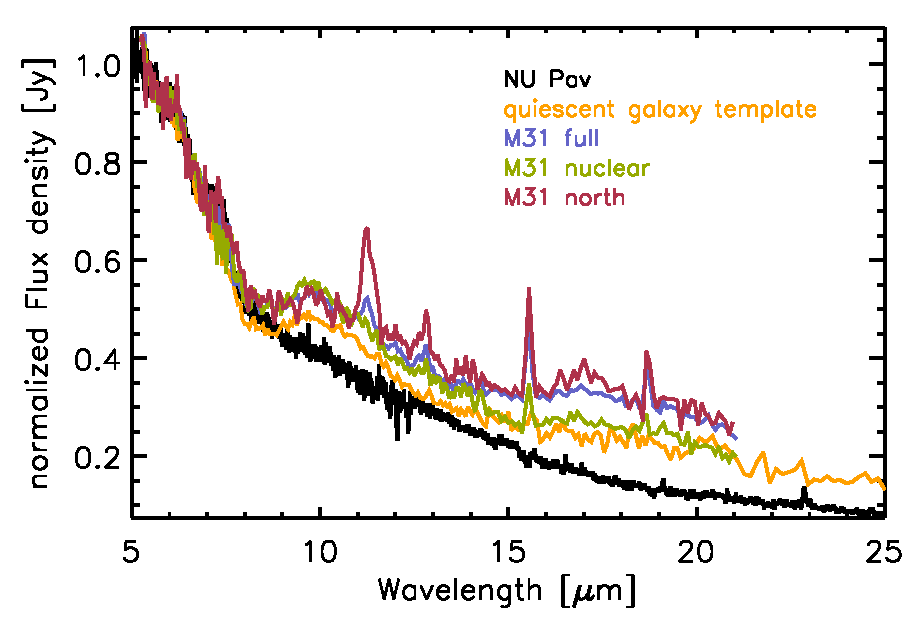
\includegraphics[width = 8 cm]{./fig12.eps}
\caption{The spectra of the M31 nucleus (nuclear, north and full) compared with the M giant $\nu$ Pav and the quiescent galaxy template of \citet{Kaneda:08}, normalized to the 5.4 $\mu$m flux density.}
\label{fig:nuc_stellar}
\end{figure}

% PAH emission
We investigate the PAH emission bands in the north spectrum in two ways. First, we apply PAHFIT \citep{Smith:2007lr} to the spectrum of the north region and rely on the stellar component within PAHFIT (a blackbody of 5000K) to account for the stellar contribution to the spectrum (Figure~\ref{fig:nuc_pahfit}, left). Secondly, we first subtract the stellar contribution by using the nuclear spectrum (normalized at 5.4 $\mu$m) and then apply PAHFIT to this stellar-subtracted north spectrum (Figure~\ref{fig:nuc_pahfit}, right). The continuum emission is overestimated between $\sim$ 9 to 11 $\mu$m for both methods indicating that the silicate emission may be slightly overestimated when using the nuclear spectrum and confirming that a 5000~K blackbody (the stellar component in PAHFIT) is a first-order approximation for the stellar contribution. In both cases, we further subtract the total continuum emission as found by PAHFIT and compare the residuals to a typical PAH emission spectrum as exemplified by the HII-type galaxy NGC0337 \citep{Smith:2007lr}. PAH emission is clearly detected at 11.3 $\mu$m and at 15-20~$\mu$m while it is weak or absent at 6--9 $\mu$m. The possible 6--9 $\mu$m PAH emission is distinct when applying these two methods. When using the stellar component of PAHFIT, a 6.2 $\mu$m PAH emission is present while no significant 7.7 and 8.6 $\mu$m emission is present. In contrast, when using the normalized nuclear spectrum as the stellar component, the 6.2 and 8.6 $\mu$m PAH emission is largely absent and the 7.7 $\mu$m PAH emission is weak. Hence, it is fair to conclude that the north spectrum does not show typical PAH emission. This is confirmed by looking at the PAH intensity ratios found by PAHFIT: the 7.7/11.2 $\mu$m PAH intensity ratio is 0.79 for {\bf the M31 north spectrum} which is much lower than the average in the SINGS sample \citep[3.6,][]{Smith:2007lr}. As mentioned, the two methods do not agree regarding the 6.2 $\mu$m band, resulting in 6.2/11.2 $\mu$m PAH intensity ratios of 1.18 and 0.14 (for the PAHFIT and nuclear stellar component respectively) whereas the SINGS average is 1.1 \citep{Smith:2007lr}. In contrast, the 17/11.2 $\mu$m PAH intensity ratios are 0.46 and 0.52 (for the PAHFIT and nuclear stellar component respectively), which is consistent with the SINGS average of 0.53 \citep{Smith:2007lr}. Similar atypical PAH emission has been detected towards elliptical galaxies \citep[e.g.][]{Kaneda:08, Vega:10} and in some low-luminosity active galactic nuclei (LLAGN) reported by \citet{Smith:2007lr}.  {\bf I wonder if this last sentence should go in the next paragraph?}


\begin{figure*}
\centering
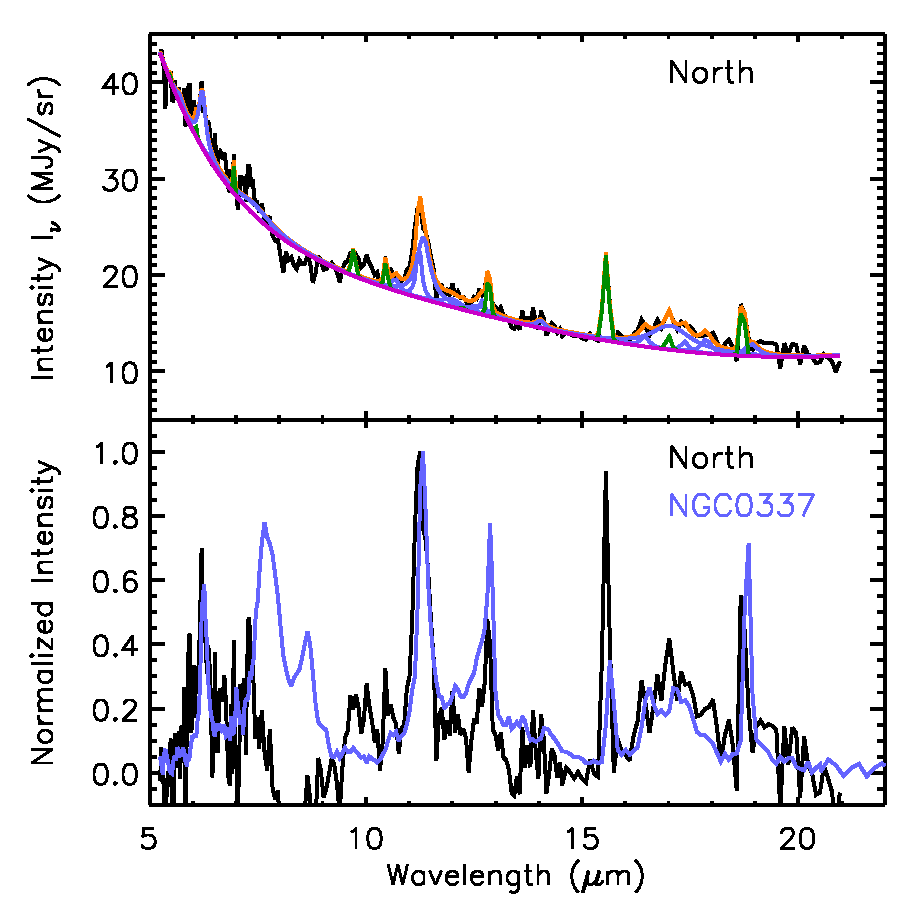
\includegraphics[width = 8 cm]{./fig13a.eps}
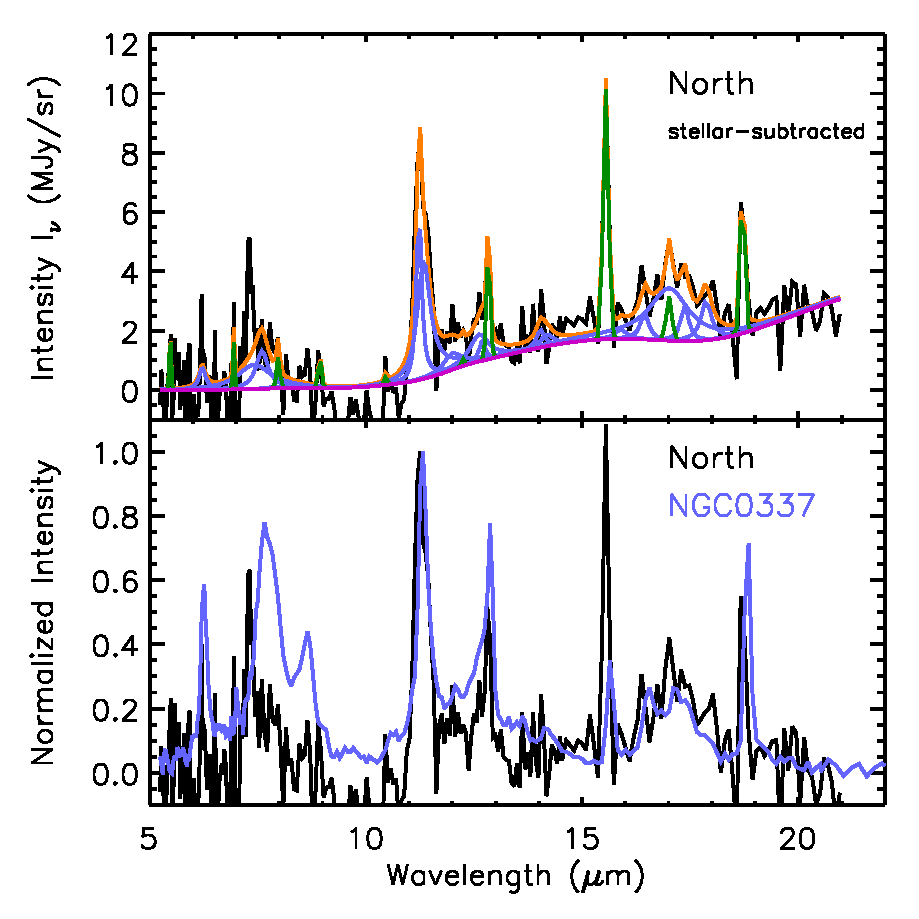
\includegraphics[width = 8 cm]{./fig13b.eps}
\caption{(top) PAHFIT result for the M31 north spectrum (left) and the M31 north spectrum subtracted by the stellar component (as defined by the M31 nuclear spectrum, right): fit (orange), continuum (magenta), individual dust components (blue), individual fine-structure lines and H$_2$ lines (green). (bottom) Continuum subtracted spectra of the north region (left) and the north region without the stellar component (right) compared with that of the HII-type galaxy NGC0337 \citep{Smith:2007lr}, normalized to the peak intensity of the  11.2~$\mu$m PAH emission. }
\label{fig:nuc_pahfit}
\end{figure*}

To place M31 in the context of other galaxies,
Figure \ref{smithspec} compares the full 30\arcsec $\times$ 50\arcsec\ M31 nuclear spectrum with the 
%spectra extracted from the smaller regions in the centre and the North (inset, top and bottom). Also shown are 
nuclear spectra of similar spectral shape from six SINGS galaxies \citep{Smith:2007lr}.% 
\footnote{The IRS spectra for the SINGS galaxies were extracted over areas ranging from 2 to 8 kpc$^2$, whereas the M31 spectrum covers a much smaller area (0.02~kpc$^2$).}
All 6 SINGS galaxies share similar PAH feature characteristics to the M31 spectrum ({\bf e.g. weak 6--8~$\mu$m features}) but none of them contains obvious silicate emission. 
%Although \citet{Mason2012} reported silicate emission towards NGC4594. However, the decrease in surface brightness levels off around $\sim$ 8 $\mu$m, similar as for the full and north spectrum of M31, and thus the silicate emission may be present nevertheless. 
%All of these comparison galaxies have some type of LLAGN. 
The SINGS galaxies with similar spectral shapes include  three elliptical galaxies, two spirals, and a lenticular; there is some disagreement over the exact nuclear spectral types of these six galaxies \citep{kennicutt03,Smith:2007lr, moustakas2010}.  All are classified as some form of LLAGN
such as Seyfert or LINER \citep[luminous AGNs were intentionally omitted from the SINGS sample;][]{kennicutt03}, although they are
by no means the only LLAGNs in the SINGS sample.
%Published estimates of the black hole masses for these galaxies range from $1.5-5.5\times10^{8}$~M$_{\sun}$
%\citep[for NGC~1316 and NGC~4595, respectively]{nowak08, kormendy88}, or about $1-4\times$ that of M31.
%M81 is classified as a LINER, with a black hole mass of $7\times10^7$~M$_{\sun}$ \citep{devereux03}.
\citet{Li09} concluded that the central black hole in M31 (M31*) is currently inactive, with direct observational signatures seen only
at radio and X--ray wavelengths, so finding additional signatures in the mid-infrared is of great interest.
To our knowledge, no such signatures have been reported; broadband mid-infrared imaging of the central 
regions of M31 \citep{davidge06,Barmby2006lr} did not identify unambiguous nuclear emission. The bluest
part of the spectrum in Figure~\ref{smithspec} is dominated by the continuum, in agreement with the
expectation that stellar light dominates at these wavelengths.


Could radiation from M31* be responsible for the suppression of the  6--8~$\mu$m PAH features compared
to the 11.3~$\mu$m feature?
As discussed by  \citet{Smith:2007lr} and \citet{Smith2010}, inferring such a suppression must be done with caution, 
because the 6--8~$\mu$m features are more susceptible to dilution by the stellar continuum. 
Several connections between PAH suppression and the presence of an AGN are possible, including destruction of small PAH molecules by a hard radiation field, modification of the structure of the PAH molecules, or weak ultraviolet continuum from low star formation rates 
leading to decreased PAH excitation \citep{Smith:2007lr, Diamond2010}.  In the latter case, the AGN is not the cause of the suppressed  6--8~$\mu$m features but rather is only detectable when the nuclear star formation rate is low.
Previous work has found low rates of star formation in the centre of M31: although \citet{Melchior2013} found a significant 
amount of cold gas in the centre of the galaxy, this gas does not appear to be associated with current star formation \citep[see also][]{Li09}.
In modelling the far-infrared spectral energy distribution, \cite{Groves2012} found that  
the old stellar population in the M31 bulge is sufficient to heat the observed dust; no young stellar population is needed. As shown, the nuclear spectrum is dominated by the stellar component and the dust continuum may only be weakly  present at the longer wavelengths. This is consistent with a low star formation rate. We conclude that PAH feature ratios cannot provide direct evidence for radiation from M31*.






